\documentclass{beamer}

\let\NOTARTICLE=1
\let\BEAMER=1
\let\FEWFONTS=1

\newenvironment{theindex}
 {\let\item\par
  %definitions for subitem etc
  }{}
\newcommand\indexspace{}

\usepackage[utf8]{inputenc}

\usepackage{graphicx} % support the \includegraphics command and options

\usepackage{parskip} % Activate to begin paragraphs with an empty line rather than an indent

%%% PACKAGES
\usepackage{booktabs} % for much better looking tables
\usepackage{array} % for better arrays (eg matrices) in maths
\ifdefined\BEAMER
\else
\usepackage{paralist} % very flexible & customisable lists (eg. enumerate/itemize, etc.)\prefix\t$.
\fi
\usepackage{verbatim} % adds environment for commenting out blocks of text & for better verbatim
\ifdefined\BEAMER
\else
\ifdefined\THESIS
\usepackage{subcaption}
\else
\usepackage{subfig} % make it possible to include more than one captioned figure/table in a single float
\fi
\fi
\usepackage{mathtools} % for the all important \coloneqq symbol
\usepackage{hyperref} % for hyperreferences
\usepackage{IEEEtrantools} % for \IEEEeqnarray
\usepackage{pbox} % for \pbox
\usepackage{multirow,bigdelim} % for \multirow
\usepackage{lettrine} % For the drop cap
\usepackage{mathpartir} % for \inferrule, \inferrule* and the mathpar environment
\usepackage{listings}

\usepackage{caption}
\captionsetup{singlelinecheck=off}

\ifdefined\NOTARTICLE
\else

%%% ToC (table of contents) APPEARANCE
\usepackage[nottoc,notlof,notlot]{tocbibind} % Put the bibliography in the ToC
\usepackage[titles,subfigure]{tocloft} % Alter the style of the Table of Contents
\renewcommand{\cftsecfont}{\rmfamily\mdseries\upshape}
\renewcommand{\cftsecpagefont}{\rmfamily\mdseries\upshape} % No bold!

\fi

%% Font things %%
\usepackage{amssymb}
\usepackage{cmll} % Linear logic symbols!
\ifdefined\FEWFONTS
\else
\usepackage{bm} % for bold Greek letters
\fi
\usepackage{stmaryrd}
\usepackage{bbm}

%% Get the sqsubsetneqq character from the mathabx package
\DeclareFontFamily{U}{mathb}{\hyphenchar\font45}
\DeclareFontShape{U}{mathb}{m}{n}{
      <5> <6> <7> <8> <9> <10> gen * mathb
      <10.95> mathb10 <12> <14.4> <17.28> <20.74> <24.88> mathb12
      }{}
\DeclareSymbolFont{mathb}{U}{mathb}{m}{n}

\DeclareMathSymbol{\sqsubsetneq}    {3}{mathb}{"88}
\DeclareMathSymbol{\varsqsubsetneq} {3}{mathb}{"8A}
\DeclareMathSymbol{\varsqsubsetneqq}{3}{mathb}{"92}
\DeclareMathSymbol{\sqsubsetneqq}   {3}{mathb}{"90}

%% Get the left and right moons from the wasysym package

\DeclareFontFamily{U}{wasy}{}
\DeclareFontShape{U}{wasy}{m}{n}{ <5> <6> <7> <8> <9> gen * wasy
      <10> <10.95> <12> <14.4> <17.28> <20.74> <24.88>wasy10  }{}
\DeclareFontShape{U}{wasy}{b}{n}{ <-10> sub * wasy/m/n
 <10> <10.95> <12> <14.4> <17.28> <20.74> <24.88>wasyb10 }{}
\DeclareFontShape{U}{wasy}{bx}{n}{ <-> sub * wasy/b/n}{}

\def\wasyfamily{\fontencoding{U}\fontfamily{wasy}\selectfont}
\def\leftmoon   {\mbox{\wasyfamily\char36}}
\def\rightmoon  {\mbox{\wasyfamily\char37}}

%% Lists %%
\usepackage{enumerate}

%% Graphics %%
\usepackage{tikz}
\usetikzlibrary{cd}
\usetikzlibrary{patterns}
\usetikzlibrary{calc}
\usetikzlibrary{decorations.pathmorphing}
\usetikzlibrary{positioning}

\tikzset{inlinearrows/.style={anchor=base,baseline,x=0.6\baselineskip,y=0.6\baselineskip}}

\ifdefined\BEAMER
\else

%% Theorems! %%
\usepackage{amsthm}
\theoremstyle{plain} % Theorems, lemmas, propositions etc.
\newtheorem{theorem}{Theorem}[section]
\newtheorem{lemma}[theorem]{Lemma}
\newtheorem{proposition}[theorem]{Proposition}
\newtheorem{corollary}[theorem]{Corollary}
\newtheorem{fact}[theorem]{Fact}
\newtheorem{construction}[theorem]{Construction}
\theoremstyle{definition} % Definitions etc.  
\newtheorem{definition}[theorem]{Definition}
\newtheorem{notation}[theorem]{Notation}
\theoremstyle{remark} % Remarks
\newtheorem{remark}[theorem]{Remark}
\newtheorem{remarks}[theorem]{Remarks}
\newtheorem{example}[theorem]{Example}
\newtheorem{question}[theorem]{Question}
\newtheorem{slogan}[theorem]{Slogan}

\newtheoremstyle{note} {3pt} {3pt} {\itshape} {} {\itshape} {:} {.5em} {} % For short notes
\theoremstyle{note}
\newtheorem{note}[theorem]{Note}

\fi

%% Exercises and answers %%
\usepackage{answers}

\newtheoremstyle{exercisestyle}% name
  {6pt}   % ABOVESPACE
  {6pt}   % BELOWSPACE
  {\itshape}  % BODYFONT
  {0pt}       % INDENT (empty value is the same as 0pt)
  {\bfseries} % HEADFONT
  {.}         % HEADPUNCT
  {3pt} % HEADSPACE
  {}          % CUSTOM-HEAD-SPEC

\theoremstyle{exercisestyle}
\newtheorem{exercise}{Exercise}
\newtheorem{answerthm}{Exercise}

\Newassociation{answer}{answerthm}{answers}
\newcommand{\answerthmparams}{}

%% Changes to enumerate things so they look better %%\sigma$

\makeatletter
\def\enumfix{%
\if@inlabel
 \noindent \par\nobreak\vskip-\topsep\hrule\@height\z@
\fi}

\let\olditemize\itemize
\def\itemize{\enumfix\olditemize}
\let\oldenumerate\enumerate
\def\enumerate{\enumfix\oldenumerate}

%% Random crap %%
\usepackage{xifthen}

\makeatletter
\def\thm@space@setup{%
  \thm@preskip=\parskip \thm@postskip=0pt
}
\makeatother

\makeatletter
\newcommand*{\relrelbarsep}{.386ex}
\newcommand*{\relrelbar}{%
  \mathrel{%
    \mathpalette\@relrelbar\relrelbarsep
  }%
}
\newcommand*{\@relrelbar}[2]{%
  \raise#2\hbox to 0pt{$\m@th#1\relbar$\hss}%
  \lower#2\hbox{$\m@th#1\relbar$}%
}
\providecommand*{\rightrightarrowsfill@}{%
  \arrowfill@\relrelbar\relrelbar\rightrightarrows
}
\providecommand*{\leftleftarrowsfill@}{%
  \arrowfill@\leftleftarrows\relrelbar\relrelbar
}
\providecommand*{\xrightrightarrows}[2][]{%
  \ext@arrow 0359\rightrightarrowsfill@{#1}{#2}%
}
\providecommand*{\xleftleftarrows}[2][]{%
  \ext@arrow 3095\leftleftarrowsfill@{#1}{#2}%
}
\makeatother

\newcommand{\catname}[1]{{\normalfont\textbf{#1}}}
\newcommand{\Rings}{\catname{CRing}}
\newcommand{\CAT}{\catname{CAT}}
%\newcommand{\Top}{\catname{Top}}
\newcommand{\Set}{\catname{Set}}
\newcommand{\Cat}{\catname{Cat}}
\newcommand{\MonCat}{\catname{MonCat}}
\newcommand{\SymmMonCat}{\catname{SymmMonCat}}
\newcommand{\Cont}{\catname{Cont}}
\newcommand{\Sch}{\catname{Sch}}
\newcommand{\Rel}{\catname{Rel}}
\newcommand{\Mod}[1][]{\ifthenelse{\isempty{#1}}{\catname{Mod}}{#1\catname{mod}}}
\DeclareMathOperator{\sh}{Sh}
\newcommand{\Sh}[1][]{\ifthenelse{\isempty{#1}}{\sh}{\sh(#1)}}
\newcommand{\map}[3]{#2\xrightarrow{#1} #3}
\newcommand*\from{\colon}
\newcommand*\bigto{\Rightarrow}
\newcommand{\cmap}[3]{#1\from{}#2\to{}#3}
\newcommand\oppcat[1]{#1^{\mathrm{op}}}
\newcommand{\object}{\colon}
\DeclareRobustCommand{\vmap}[3] {\begin{tikzcd} #2 \arrow[d, "#1"] \\ #3 \end{tikzcd}}
\newcommand{\partref}[1]{(\ref{#1})}
\newcommand{\intgrpd}[4] {#1 \xrightrightarrows[#3]{#4} #2}
\DeclareRobustCommand{\bigintgrpd}[4] {\begin{tikzcd}[ampersand replacement=\&] #1 \arrow[r, shift left=0.5ex, "#3"] \arrow[r, shift right=0.5ex, "#4"'] \& #2 \end{tikzcd}}

\usepackage{xspace}

\newcommand{\etale}{\'{e}tale\xspace}
\newcommand{\Etale}{\'{E}tale\xspace}

\def \inv {^{-1}}

\DeclareMathOperator{\id}{id}
\DeclareMathOperator{\op}{op}
\DeclareMathOperator{\pr}{pr}
\DeclareMathOperator{\inj}{in}
\DeclareMathOperator{\pre}{{pre}}
\DeclareMathOperator{\et}{{\acute{e}t}}

\DeclareMathOperator{\Hom}{Hom}
\DeclareMathOperator{\Spec}{Spec}

\DeclareMathOperator{\ol}{ol}

\def\presuper#1#2%
  {\mathop{}%
   \mathopen{\vphantom{#2}}^{#1}%
   \kern-\scriptspace%
   #2}
\def\presub#1#2%
  {\mathop{}%
   \mathopen{\vphantom{#2}}_{#1}%
   \kern-\scriptspace%
   #2}

\newsavebox{\overlongequation}
\newenvironment{longdiagram}
 {\begin{displaymath}\begin{lrbox}{\overlongequation}$\displaystyle}
 {$\end{lrbox}\makebox[0pt]{\usebox{\overlongequation}}\end{displaymath}}

%% Our things %%

\newcommand{\neggame}[1]{\presuper{\perp}{#1}}
\newcommand{\tensor}{\otimes}
\newcommand{\Tensor}{\bigotimes}
\newcommand{\sequoid}{\oslash}
\newcommand{\varsequoid}{\vartriangleleft}
\renewcommand{\implies}{\multimap}
\newcommand{\iimpl}{\Longrightarrow}
\newcommand{\comp}[2]{#1 \circ #2}
\newcommand{\icomp}[2]{\comp{#1}{#2}}
\newcommand{\cprd}{\sqcup}
\newcommand{\bigcprd}{\bigsqcup}
\newcommand{\G}{\mathcal G}
\newcommand{\W}{\mathcal W}
\newcommand{\suchthat}{\;\colon\;}
\newcommand{\varsuchthat}{\;\mid\;}
\newcommand{\esuchthat}{\;.\;}
\newcommand{\OP}{\{O,P\}}
\newcommand{\QA}{\{Q,A\}}
\renewcommand{\L}{\mathcal L}
\newcommand{\F}{\mathcal F}
\newcommand{\U}{\mathcal U}
\newcommand{\s}{\mathfrak s}
\renewcommand{\t}{\mathfrak t}
\renewcommand{\u}{\mathfrak u}
\renewcommand{\d}{\mathfrak d}
\newcommand{\e}{\mathfrak e}
\newcommand{\emptyplay}{\epsilon}
\newcommand{\bracketed}[1]{\left({#1}\right)}
\newcommand{\bneggame}[1]{{\bracketed{\neggame{#1}}}}
\newcommand{\prefix}{\sqsubseteq}
\newcommand{\ppprefix}{\sqsubset}
\newcommand{\pprefix}{\sqsubsetneqq}
\renewcommand{\ss}{\mathbf{s}}
\newcommand{\bN}{\mathbb{N}}
\newcommand{\bC}{\mathbb{C}}
\newcommand{\bB}{\mathbb{B}}
\newcommand{\bP}{\mathbb{P}}
\newcommand{\pfun}{\rightharpoonup}
\newcommand{\grel}[1]{\underline{#1}}
\DeclareMathOperator{\length}{length}
\renewcommand{\b}{\mathfrak b}
\renewcommand{\r}{\mathfrak r}
\newcommand{\bbeta}{{\bm{\beta}}}
\newcommand{\st}{{\Sigma^*}}
\let\sec\S
\renewcommand{\S}{{\mathfrak{S}}}
\DeclareMathOperator{\cc}{cc}
\DeclareMathOperator{\subs}{subs}
\DeclareMathOperator{\ret}{ret}
\DeclareMathOperator{\zz}{zz}
\newcommand{\aaa}{\mathbf{a}}
\newcommand{\bbb}{\mathbf{b}}
\newcommand{\ccc}{\mathbf{c}}
\newcommand{\ddd}{\mathbf{d}}
\newcommand{\B}{\mathcal B}
\newcommand{\BB}{\mathbf B}
\renewcommand{\H}{\mathcal H}
\DeclareMathOperator{\assoc}{assoc}
\DeclareMathOperator{\lunit}{lunit}
\DeclareMathOperator{\runit}{runit}
\DeclareMathOperator{\dom}{dom}
\DeclareMathOperator{\sym}{sym}
\newcommand{\braid}{\sym}
\newcommand{\blank}{\,\underline{\hspace{1.5ex}}\,}
\DeclareMathOperator{\cn}{cn}
\newcommand{\impliescn}{\protect\overset{\cn}{\implies}}
\newcommand{\C}{{\mathcal{C}}}
\newcommand{\D}{{\mathcal{D}}}
\newcommand{\E}{{\mathcal{E}}}
\newcommand{\V}{{\mathcal{V}}}
\newcommand{\EE}{{\mathbf{E}}}
\DeclareMathOperator{\ev}{ev}
\newcommand{\der}{{\mathtt{der}}}
\newcommand{\mult}{{\mathtt{mult}}}
\DeclareMathOperator{\wk}{wk}
\newcommand{\toisom}{{\xrightarrow{\cong}}}
\DeclareMathOperator{\passoc}{{\mathsf{passoc}}}
\DeclareMathOperator{\pcomm}{{\mathsf{pcomm}}}
\DeclareMathOperator{\run}{{\mathsf{r}}}
\DeclareMathOperator{\lun}{{\mathsf{l}}}
\newcommand{\fcoal}[1]{{\leftmoon #1 \rightmoon}}
\DeclareMathSymbol{\co}{\mathord}{operators}{"3C}
\DeclareMathSymbol{\nw}{\mathord}{operators}{"3E}
\newcommand{\T}{\mathfrak{T}}
\renewcommand{\subset}{\subseteq}
\newcommand{\Ord}{\catname{Ord}}
\newcommand{\FS}{\mathcal{FS}}
\DeclareMathOperator{\rank}{rank}
\DeclareMathOperator{\dist}{{\mathsf{dist}}}
\DeclareMathOperator{\dec}{{\mathsf{dec}}}
\DeclareMathOperator{\str}{str}
\DeclareMathOperator{\weak}{weak}
\DeclareMathOperator{\Strat}{Strat}
\DeclareMathOperator{\OppStrat}{OppStrat}
\newcommand{\seqs}[1]{{\overline{{#1}^{*}}}}
\def\flushRight{\leftskip0pt plus 1fill\rightskip0pt}
\def\Centering{\relax\ifvmode\centering\fi}
\newcommand{\deno}[1]{\left\llbracket#1\right\rrbracket}
\newcommand{\converges}{\Downarrow}
\newcommand{\diverges}{\Uparrow}
\newcommand{\mustconverge}{\converges^{\text{must}}}
\newcommand{\Iflt}{\mathtt{If{<}\;}}
\newcommand{\Ifgt}{\mathtt{If{>}\;}}
\newcommand{\inr}{{\mathsf{inr}}}
\newcommand{\inl}{{\mathsf{inl}}}
\newcommand{{\Na}}{\bN}
\newcommand{{\cell}}{{\mathsf{cell}}}
\newcommand{\fix}{{\mathsf{fix}}}
\newcommand{\eq}{{\mathsf{eq}}}
\DeclareMathOperator{\CCom}{CCom}
\newcommand{\power}{\mathfrak P}

% Slanty things
\newcommand*{\xslant}[2][76]{%
  \begingroup
    \sbox0{#2}%
    \pgfmathsetlengthmacro\wdslant{\the\wd0 + cos(#1)*\the\wd0}%
    \leavevmode
    \hbox to \wdslant{\hss
      \tikz[
        baseline=(X.base),
        inner sep=0pt,
        transform canvas={xslant=cos(#1)},
      ] \node (X) {\usebox0};%
      \hss
      \vrule width 0pt height\ht0 depth\dp0 %
    }%
  \endgroup
}

\makeatletter
\newcommand*{\xslantmath}{}
\def\xslantmath#1#{%
  \@xslantmath{#1}%
}
\newcommand*{\@xslantmath}[2]{%
  % #1: optional argument for \xslant including brackets
  % #2: math symbol
  \ensuremath{%
    \mathpalette{\@@xslantmath{#1}}{#2}%
  }%
}
\newcommand*{\@@xslantmath}[3]{%
  % #1: optional argument for \xslant including brackets
  % #2: math style
  % #3: math symbol
  \xslant#1{$#2#3\m@th$}%
}
\makeatother

\newcommand{\seqdeno}[1]{\xslantmath{\llbracket}#1\xslantmath{\rrbracket}}

% Empty set etc.

\let\oldemptyset\emptyset
\let\emptyset\varnothing

%% Constant width xrightarrows
\newlength{\arrow}
\settowidth{\arrow}{\scriptsize$1000$}
\newcommand*{\constantwidthxrightarrow}[1]{\xrightarrow{\mathmakebox[\arrow]{#1}}}

%% Landscape pages
\usepackage{everypage}
\usepackage{environ}
\usepackage{pdflscape}
\newcounter{abspage}

\ifdefined\NOTARTICLE

\else

\makeatletter
\newcommand{\newSFPage}[1]% #1 = \theabspage
  {\global\expandafter\let\csname SFPage@#1\endcsname\null}

\NewEnviron{SidewaysFigure}{\begin{figure}[p]
\protected@write\@auxout{\let\theabspage=\relax}% delays expansion until shipout
  {\string\newSFPage{\theabspage}}%
\ifdim\textwidth=\textheight
  \rotatebox{90}{\parbox[c][\textwidth][c]{\linewidth}{\BODY}}%
\else
  \rotatebox{90}{\parbox[c][\textwidth][c]{\textheight}{\BODY}}%
\fi
\end{figure}}

\AddEverypageHook{% check if sideways figure on this page
  \ifdim\textwidth=\textheight
    \stepcounter{abspage}% already in landscape
  \else
    \@ifundefined{SFPage@\theabspage}{}{\global\pdfpageattr{/Rotate 0}}%
    \stepcounter{abspage}%
    \@ifundefined{SFPage@\theabspage}{}{\global\pdfpageattr{/Rotate 90}}%
  \fi}
\makeatother

\fi

%% PCF Things

\newcommand{\nat}{{\mathtt{nat}}}
\newcommand{\bool}{{\mathtt{bool}}}

\newcommand{\Y}{\mathbf{Y}}
\newcommand{\opto}{\longrightarrow}
\newcommand{\oopto}{\dashrightarrow}
\newcommand{\n}{{\mathtt{n}}}
\DeclareMathOperator{\IfO}{{\mathsf{If0}}}
\DeclareMathOperator{\suc}{{\mathsf{succ}}}
\DeclareMathOperator{\pred}{{\mathsf{pred}}}
\newcommand{\0}{{\mathtt{0}}}

\newcommand{\iter}{{\mathtt{iter}}}
\newcommand{\rec}{\iter}
\newcommand{\Var}{{\mathtt{Var}}}
\DeclareMathOperator{\Varr}{Var}
\newcommand{\new}{{\mathtt{new}}}
\newcommand{\case}{{\mathtt{case}}}

\newcommand{\lmam}{\mathrel{\sqsubseteq_{m\&m}}}
\newcommand{\emam}{\mathrel{\equiv_{m\&m}}}
\newcommand{\lst}{\mathrel{\lesssim}}
\newcommand{\smam}{\mathrel{\sim_{m\&m}}}
\newcommand{\amam}{\mathrel{\approx_{m\&m}}}

\newcommand{\oes}{\sim}

%% Idealized Algol things

\newcommand{\com}{{\mathtt{com}}}
\newcommand{\skipp}{{\mathsf{skip}}}
\DeclareMathOperator{\seq}{{\mathsf{seq}}}
\DeclareMathOperator{\neww}{{\mathsf{new}}}
\DeclareMathOperator{\mkvar}{{\mathsf{mkvar}}}
\newcommand{\deref}{\texttt{@}}
\DeclareMathOperator{\dereff}{\mathsf{deref}}
\DeclareMathOperator{\assign}{\mathsf{assign}}
\newcommand{\ia}[2]{\langle #1 , #2 \rangle}
\newcommand{\stup}[3]{\langle #1 \mid #2 \mapsto #3 \rangle}

%% Hyland-Ong games things

\newbox\gnBoxA
\newdimen\gnCornerHgt
\setbox\gnBoxA=\hbox{$\ulcorner$}
\global\gnCornerHgt=\ht\gnBoxA
\newdimen\gnArgHgt
\def\pv #1{%
    \setbox\gnBoxA=\hbox{$#1$}%
    \gnArgHgt=\ht\gnBoxA%
    \ifnum     \gnArgHgt<\gnCornerHgt \gnArgHgt=0pt%
    \else \advance \gnArgHgt by -\gnCornerHgt%
    \fi \raise\gnArgHgt\hbox{$\ulcorner$} \box\gnBoxA %
    \raise\gnArgHgt\hbox{$\urcorner$}}
\def\ov #1{%
    \setbox\gnBoxA=\hbox{$#1$}%
    \gnArgHgt=\ht\gnBoxA%
    \ifnum     \gnArgHgt<\gnCornerHgt \gnArgHgt=0pt%
    \else \advance \gnArgHgt by -\gnCornerHgt%
    \fi \raise\gnArgHgt\hbox{$\llcorner$} \box\gnBoxA %
    \raise\gnArgHgt\hbox{$\lrcorner$}}
\newcommand{\ct}[1]{\lceil#1\rceil}
\DeclareMathOperator{\Int}{int}

%% Nondeterministic Factorization things

\newcommand{\code}{\mathsf{code}}
\newcommand{\Det}{\mathsf{Det}}

%% Flexible strategy things

\newcommand{\stle}{{\;\le_s\;}}
\newcommand{\steq}{{\;=_s\;}}
\newcommand{\exle}{\sqsubseteq}
\newcommand{\exlub}{\bigsqcup}
\newcommand{\dv}{{\text{\lightning}}}
\DeclareMathOperator{\pocl}{pocl}
\newcommand{\plot}{\mathrel{\triangleleft}}
\newcommand{\shad}{\mathfrak{S}}
%\newcommand{\tree}{\mathfrak{T}}
\newcommand{\Tau}{T}
\newcommand{\Epsilon}{E}
\newcommand{\sw}{\triangleleft}

%% Roman numerals

\newcommand{\RN}[1]{%
  \textup{\uppercase\expandafter{\romannumeral#1}}%
}
\newcommand{\RNl}[1]{%
  \mathrel{\raisebox{1pt}{$\overline{\underline{#1}}$}}
}

%% Game language things

\newcommand{\ul}[1]{{\underline{#1}}}
\newcommand{\A}{{\mathcal{A}}}
\renewcommand{\P}{\mathcal P}
\newcommand{\M}{\mathcal M}
\newcommand{\N}{\mathcal N}
\newcommand{\X}{\mathcal X}
\newcommand{\YY}{\mathcal Y}
\newcommand{\hole}{\blank}
\newcommand{\Tct}{\xrightarrow{T}t}
\newcommand{\teamconverge}[2]{\xrightarrow{#1}#2}

%% Inference rule things
\newcommand{\rulename}[1]{\LeftTirNameStyle{#1}}
\newcommand{\ts}{\mathbin{\vdash}}
\newcommand{\nts}{\mathbin{\not\vdash}}

%% Double category things
\newcommand{\hc}[2]{\left({#1}\middle|{#2}\right)}
\newcommand{\vc}[2]{\left(\frac{#1}{#2}\right)}

%% What is going on?
\DeclareMathOperator{\Kl}{Kl}
\DeclareMathOperator{\Mell}{Mell}
\newcommand{\powerset}{\mathcal P}
\DeclareMathOperator{\ask}{{\mathsf{ask}}}
\newcommand{\sleep}{{\mathsf{sleep}}}
\newcommand{\true}{\mathbbm{t}}
\newcommand{\false}{\mathbbm{f}}
\DeclareMathOperator{\If}{\mathsf{If}}
\newcommand{\Then}{\mathrel{\mathsf{then}}}
\newcommand{\Else}{\mathrel{\mathsf{else}}}
\newcommand\cat{\mathbin{+\mkern-10mu+}}

%% Profunctor arrows

\makeatletter
\def\slashedarrowfill@#1#2#3#4#5{%
  $\m@th\thickmuskip0mu\medmuskip\thickmuskip\thinmuskip\thickmuskip
   \relax#5#1\mkern-7mu%
   \cleaders\hbox{$#5\mkern-2mu#2\mkern-2mu$}\hfill
   \mathclap{#3}\mathclap{#2}%
   \cleaders\hbox{$#5\mkern-2mu#2\mkern-2mu$}\hfill
   \mkern-7mu#4$%
}
\def\rightslashedarrowfill@{%
  \slashedarrowfill@\relbar\relbar\mapstochar\rightarrow}
\newcommand\xslashedrightarrow[2][]{%
  \ext@arrow 0055{\rightslashedarrowfill@}{#1}{#2}}
\makeatother
\newcommand{\pto}{{\xslashedrightarrow{} }}

%% Profunctors 
\DeclareMathOperator{\Prof}{Prof}
\DeclareMathOperator{\End}{End}
\DeclareMathOperator{\Endoprof}{Endoprof}

%% Our

\def\searchmacro#1{
  \AtBeginOfFiles{%
    \ifdefined#1
      \expandafter\def\csname \currfilename:found\endcsname{}%
    \fi}
  \AtEndOfFiles{%
    \ifdefined#1
      \unless\ifcsname \currfilename:found\endcsname
        \immediate\write\finder{found in '\currfilename'}%
    \fi\fi}}

%% Isomorphism arrows on commutative diagrams %%
\tikzset{Isom/.style={every to/.append style={edge node={node [sloped, above, allow upside down, auto=false]{$\cong$}}}},
         Isom'/.style={every to/.append style={edge node={node [sloped, above, allow upside down, auto=false, rotate=180]{$\cong$}}}},
         Sim/.style={every to/.append style={edge node={node [sloped, above, allow upside down, auto=false]{$\sim$}}}},
         Sim'/.style={every to/.append style={edge node={node [sloped, above, allow upside down, auto=false, rotate=180]{$\sim$}}}}}

%% Adjunctions
\newcommand{\adjunction}[4]{%
  {#1} \underset{\underset{#3}{\longleftarrow}}{\overset{\overset{#2}{\longrightarrow}}{\bot}} {#4}}        

%% Important!
\newcommand\Mellies{Melli\`{e}s\xspace}

\makeatletter
\newcommand{\colim@}[2]{%
  \vtop{\m@th\ialign{##\cr
    \hfil$#1\operator@font colim$\hfil\cr
    \noalign{\nointerlineskip\kern1.5\ex@}#2\cr
    \noalign{\nointerlineskip\kern-\ex@}\cr}}%
}
\newcommand{\colim}{%
  \mathop{\mathpalette\colim@{\rightarrowfill@\textstyle}}\nmlimits@
}
\makeatother

\makeatletter
\newcommand{\laxcolim@}[2]{%
  \vtop{\m@th\ialign{##\cr
    \hfil$#1\operator@font colim_l$\hfil\cr
    \noalign{\nointerlineskip\kern1.5\ex@}#2\cr
    \noalign{\nointerlineskip\kern-\ex@}\cr}}%
}
\newcommand{\laxcolim}{%
  \mathop{\mathpalette\laxcolim@{\rightarrowfill@\textstyle}}\nmlimits@
}
\makeatother

\DeclareMathOperator{\Colim}{colim}

\DeclareMathOperator{\DG}{DG}
\DeclareMathOperator{\RV}{RV}
\newcommand{\Rv}{\catname{Rv}}

\let\choose\undefined
\DeclareMathOperator{\choose}{\mathsf{choose}}
\DeclareMathOperator{\tr}{tr}
\DeclareMathOperator{\test}{test}

%% Slot game things %%
\newcommand{\circled}[1]{\raisebox{.5pt}{\textcircled{\raisebox{-.9pt} {#1}}}}
\newcommand{\slot}{{\circled{\$}}}

\DeclareMathOperator{\may}{may}
\DeclareMathOperator{\must}{must}

\newcommand{\encode}[1]{\lceil#1\rceil}
\DeclareMathOperator{\app}{\mathsf{app}}
\DeclareMathOperator{\lett}{\mathsf{let}}
\newcommand{\inn}{\mathrel{\mathsf{in}}}
\DeclareMathOperator{\byval}{\mathsf{byval}}

\DeclareMathOperator{\rread}{read}
\DeclareMathOperator{\wwrite}{write}

\DeclareSymbolFont{bbsymbol}{U}{bbold}{m}{n}
\DeclareMathSymbol{\bbsemicolon}{\mathbin}{bbsymbol}{"3B}
\newcommand{\semicom}{\bbsemicolon}

\newcommand{\ms}{\makebox[-1pt]{}}

%%% END Article customizations



\newtheorem{proposition}{Proposition}

\newcommand{\sign}[1]{\\\hfill -- \parbox[t]{.3\textwidth}{#1}}
\usepackage{wasysym}
\usepackage[absolute,overlay]{textpos}
\DeclareMathOperator{\ding}{ding}

%%% END Article customizations

\title{A unified approach to the semantics of effects}
\subtitle{GaLoP 2018, Thessaloniki}

\author{John Gowers}

\AtBeginSection{\frame{\sectionpage}}
\AtBeginSubsection{\frame{\subsectionpage}}

\begin{document}

\begin{frame}
  \titlepage
\end{frame}

\begin{frame}
  \frametitle{Outline}
  \tableofcontents
\end{frame}

\section{Some Examples}

\renewcommand*{\arraystretch}{0.5}

%\begin{frame}[allowframebreaks]
  %\frametitle{Related Work}
  %\nocite{mcCHFiniteND, RusssThesis, TsukadaSheaves, RoscoeCspInfinite, LevyGsInfinite, LairdOrdinalGames}
  %\bibliographystyle{plain}
  %\bibliography{../../common/phd_bibliography}
%\end{frame}

\begin{frame}
  \frametitle{Nondeterminism and innocence}

  The game semantics of nondeterminism models nondeterministic programs by \emph{nondeterministic strategies}, where $P$ can have multiple replies to an $O$-position. But there is no satisfactory definition of an \emph{innocent} nondeterministic strategy.
  \pause

  For example, consider the term
  \[
    (\lambda f.f 0) \text{ OR } (\lambda f.f 1)
    \]
  whose denotation is the union of the denotations of the same components.  
  But this strategy is not innocent!
  \pause

  Tsukada and Ong: the problem is missing \emph{branching time information}.
\end{frame}

\begin{frame}
  \frametitle{Is there another approach?}

  Harmer's thesis: a nondeterministic innocent strategy is any strategy of the form
  \[
    1 \xrightarrow{\top_{\bB}}
    \bB \xrightarrow{\sigma}
    A
    \]
  where $\sigma$ is innocent.
  \pause

  \textit{A more “synthetic”, a priori definition
of what it is to be an innocent strategy would be preferable.}
  \sign{Harmer}
  \pause

  \textit{Such
an approach is ultimately unsatisfactory as it provides no new
  insights on nondeterministic stateless computation.}
  \sign{Tsukada, Ong}
  \pause

  \only<4->{
  \begin{textblock}{0.5}(11,4)
    \rotatebox{350}{\Large\#unsatisfactory}
  \end{textblock}
}
\pause

  Tsukada, Ong: We can solve the problem using a sheaf-based model that retains branching-time information.
  \pause

  \only<6->{
  \begin{textblock}{0.5}(11,13)
    \rotatebox{350}{\Large\#satisfactory}
  \end{textblock}
}
\end{frame}

\begin{frame}
  \frametitle{A purely formal treatment of effects}

  Idea: If we use the indirect approach, we can treat $\top_\bB$ as a purely formal symbol and say that a nondeterministic innocent strategy for a game $A$ is a deterministic innocent strategy for $\bB\to A$.
  \pause

  We don't need to mention nondeterministic strategies at all!
  \pause

  Slight drawback: this approach distinguishes strategies that are in fact identical.  
  E.g., $\deno{\lambda b.b}$ and $\deno{\lambda b.\text{not }b}\from\bB$ both denote the term $t\text{ OR }f$.
  \pause

  \begin{minipage}{0pt}
    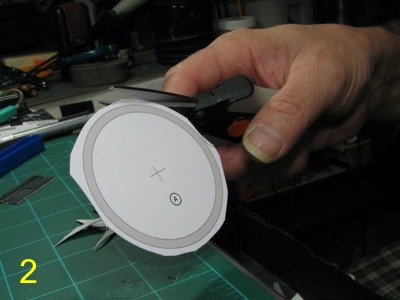
\includegraphics{circles_2.jpg}
  \end{minipage}
  \hspace{150pt}
  \begin{minipage}{0.01\textwidth}
    
\includegraphics{circles_3.jpg}
  \end{minipage}
\end{frame}

\begin{frame}
  \frametitle{The formal treatment and branching-time information}

  Clearly, the strategy $\sigma\from\bB\to A$ contains all the information about branching time that we might need if we were to reason about $\top_\bB;\sigma$.
  \pause

  Since deterministic factorization automatically holds, the problem becomes one of working out the right equivalence relation to impose on strategies for $\bN\to A$ (cutting out the circle).
  \pause

  We can use a semi-indirect approach informed by the operational semantics of the language (e.g., using linear decomposition: $\sigma,\tau\from\bB\to A$ are equivalent if and only if for all $\alpha\from\oc\bB$ there exists some $\beta\from\oc\bB$ such that $\alpha;\sigma=\beta;\tau$ -- and vice versa).
  \pause

  Or we can use more ingenious techniques.  
  For example, we can recover the Tsukada-Ong sheaf-theoretic approach by identifying $\sigma$ with the following sheaf.
  \[
    \sigma(s) = \{t\in\sigma\suchthat t\vert_A=s\}
    \]
\end{frame}

\begin{frame}
  \frametitle{Another example -- bell games}

  We want to model the language PCF${}^{\bell+}$, obtained by enlarging PCF with command types and a constant $\ding\from\com$ with the following operational semantics.
  \[
    \inferrule*[right=\bell]{ }{\ding \opto \skipp}
    \]
  ($\bell$ $=$ `ring the bell every time you evaluate this rule')
  \pause

  Game Semantics (Ghica's `slot games'): insert an additional move $\bell$ (belonging to neither player) into the play whenever we ring the bell (so $\deno{\ding}$ is the strategy with maximal play $q\bell a$).  
  
  The $\bell$s are not hidden during composition:
  \pause
  \begin{mathpar}
    \begin{array}{cccccc}
      {}    &  \com & \to & \com  & \to & \com \\
            &       &     &       &     &   q  \\
            &    q  &     &       &     &      \\
      \bell &       &     &       &     &      \\
            &    a  &     &       &     &      \\
            &       &     &   q   &     &      \\
      \bell &       &     &       &     &      \\
            &       &     &   a   &     &      \\
            &       &     &       &     &   a  \\
    \end{array}
    \and
    \rightsquigarrow
    \and
    \begin{array}{c}
      \\
      q\\
      \\
      \bell
      \\
      \\
      \bell\\
      \\
      a
    \end{array}
  \end{mathpar}
\end{frame}

\begin{frame}
  \frametitle{The formal approach to bell games}
  Suppose instead that we attempt to model $\ding$ as a purely formal morphism $1\to\bC$.  
  In our new model, a strategy for $A$ will be a strategy for $\bC\to A$ in the original model, where we interpret $\sigma\from\bC\to A$ as the strategy $\ding;\sigma\from A$.
  \pause

  For example, the term $\ding;\ding:\com$ is interpreted as the following composite.
  \[
    \bC \xrightarrow{\Delta}
    \bC \times \bC \xrightarrow{\blank;\blank}
    \bC
    \]
  \pause
  \renewcommand*{\arraystretch}{.75}
  As a a strategy:
  \[
    \begin{array}{ccc}
      \bC & \to & \bC \\
          &     &  q  \\
       q  &     &     \\
       a  &     &     \\
       q  &     &     \\
       a  &     &     \\
          &     &  a  \\
    \end{array}
    \]
\pause
$\bell$ $=$ $qa$ on the left.
\end{frame}

\begin{frame}
  \frametitle{A common theme}

  A common theme in both these examples is that formal morphisms expose moves that are normally hidden under composition.
  \pause

  For some computational effects, this is exactly what we want to do. For nondeterminism, the nondeterministic strategy approach hides too much information, and the formal approach reveals too much.
  \pause

  Topics for exploration:
  \pause

  Can we add formal morphisms $A\to A$ for all $A$ in order to make a `revealed game semantics' that is still a Cartesian closed category?
  \pause

  Are these two examples the same?  (E.g., $\ding$ = `unary nondeterminism')
  \pause

  Can we build a model of nondeterministic innocence based on bell games?
\end{frame}

\section{Cones on monoidal functors}

\begin{frame}
  We talked about formally adding morphisms into a category.  
  In this section, we'll look at a slightly more general construction.
  \pause

  The goals of this generalization are twofold:
  \pause
  \begin{itemize}
    \item To allow us to add more than one morphism at a time.
      \pause
    \item To give a more systematic account of the equivalence relation on morphisms.
  \end{itemize}
  \pause

  Previously, we wanted to add a morphism $\phi\from 1\to A$ for some object $A$ or, equivalently, a natural transformation from $I$ to the `constant $A$ functor'.
  \pause

  We replace $I$ with an arbitrary symmetric monoidal category $\C'$ and require that $\phi$ be an oplax monoidal functor.
  \pause

  Note: for every object $A$ of a CCC, the `constant $A$' functor is oplax monoidal with coherence given by the diagonal and projections.
\end{frame}

\begin{frame}
  The setup: we have an oplax monoidal functor $j\from \C'\to\C$, where $\C,\C'$ are symmetric monoidal categories.
  \pause

  We desire a symmetric monoidal category $\D$ that contains $\C$ plus additional morphisms corresponding to the image of $j$.
  \pause

  I.e., this (a \emph{$j$-category}):
  \[
    \begin{tikzcd}[row sep=large, column sep=large, ampersand replacement=\&]
      \C' \arrow[r, "()", ""'{name=term}] \arrow[d, "j"']
        \& I \arrow[d, "I"] \\
      \C \arrow[r, "J"', ""{name=J}]
        \& \D
      \arrow[Rightarrow, from=term, to=J, "\phi"]
    \end{tikzcd}\quad,
  \]
where $J$ is a lax monoidal functor and $\phi$ is a `generalized monoidal natural transformation'.
\pause

The more objects there are in $\C'$, the more morphisms there are in $\D$.  
  The more morphisms there are in $\C'$, the \emph{fewer} morphisms there are in $\D$ (or: a finer equivalence relation on morphisms).
\end{frame}

\begin{frame}
  \frametitle{The Cone on $j$}

  We can define a morphism of $j$-categories $(\D',J',\phi')\to(\D,J,\phi)$ to be an oplax monoidal functor $f\from\D'\to\D$ making the following diagram commute.
  \[
    \begin{tikzcd}[row sep=large, column sep=large, ampersand replacement=\&]
      \C' \arrow[r, "()", ""'{name=term}] \arrow[d, "j"']
        \& I \arrow[d, "I"] \\
      \C \arrow[r, "J'"'{name=Jprimedown}, ""{name=Jprime}] \arrow[d, "\id"']
        \& \D' \arrow[d, "f"] \\
      \C \arrow[r, "J", ""{name=J}]
        \& \D
      \arrow[Rightarrow, from=term, to=Jprime, shift left=1.5ex, "\phi'"]
      \arrow[Rightarrow, from=Jprimedown, to=J, shift left=1.5ex, "\id"]
      \arrow[Rightarrow, from=term, to=J, shift right=3ex, "\phi"' near end]
    \end{tikzcd}\,.
    \]
  \pause

  We get a category of $j$-categories.  
  We can show that this category has an initial object $C_j$, called the \emph{cone on $j$}.
  \pause

  $C_j$ is the category obtained from $\C$ by `formally adding morphisms $\psi_X\from I \implies jX$'.
\end{frame}

\begin{frame}
  \frametitle{Construction of $C_j$}

  The construction of $C_j$ is straightforward (and quite familiar in the Cartesian case).
  \pause

  The objects of $C_j$ are the objects of $\C$.  

  A morphism $A\to B$ in $C_j$ is a pair $(X,f)$, where $X$ is an object of $\C'$ and $f\from jX \tensor A \to B$ is a morphism in $\C'$.

  Two morphisms $(X, f)$ and $(X', f')$ are considered to be equivalent if there is some morphism $h\from X'\to X$ in $\C'$ making the following diagram commute.
  \[
    \begin{tikzcd}[ampersand replacement=\&]
      j X' \tensor A \arrow[r, "f'"] \arrow[d, "j h \tensor A"']
        \& B \\
      j X \tensor A \arrow[ur, "f"']
        \&
    \end{tikzcd}
    \]
  \pause

  Composition is given by `the only thing you can write down'.
\end{frame}

\begin{frame}
  \frametitle{Constructing models from $C_j$}

  We said that we wanted to model effects by finding a particular $j$-category $\D$ for a suitable $j$ that captures the effect in some way.
  \pause

  Even if we know nothing else about $\D$, we know that there is a functor $C_j\to\D$ that is a morphism of $j$-categories.
  \pause

  If $\D$ satisfies `$j$-factorization', then this functor is full.
  \pause

  In such a case, we can recover $\D$ by imposing a suitable equivalence relation on the morphisms in $C_j$.
  \pause

  The more morphisms we can include in $\C'$, the closer $C_j$ will be to our desired model.
\end{frame}

\section{More examples}

\begin{frame}
  \frametitle{Unbounded nondeterminism}

  Let $\G$ be the category of Hyland-Ong games.  
  \pause

  Now suppose that $\D$ is some extension of $\G$ that somehow models nondeterminism.  
  For each object $A$ of $\D$, there should be a strategy $\top_A\from 1 \to A$ that includes every position in $A$.
  \pause

  $\top_A$ is not a natural transformation $1\to\G$: this would mean that $\top_A;\sigma=\top_B$ for every $\sigma\from A \to B$.
  \pause

  However, if we require that $\sigma$ be \emph{surjective}; i.e., that every position in $B$ is the restriction of some position occurring in $\sigma$, then $\top_A;\sigma=\top_B$.  
  \pause

  If $j_s$ is the inclusion of the category $\G_s$ of games and \emph{surjective strategies} into $\G$, then $\top_A$ is a natural transformation $1\to j_s A$.
  \pause

  Therefore, $\D$ is some quotient of $C_{j_s}$.  
\end{frame}

\begin{frame}
  \frametitle{Unbounded nondeterminism and must-testing}

  $C_j$ models may-testing: in a model of unbounded nondeterminism with must-testing, we may have $\top_A;\sigma\ne \top_B$ even if $\sigma$ is surjective.  
  The reason is that $\sigma$ might have a play ending with infinitely many moves in $A$.
  \pause

  We say that a strategy $\sigma\from A \to B$ is \emph{winning} if it contains no such play.  
  Then if $j_{sw}$ is the inclusion of the category $\G_{sw}$ of games and \emph{surjective winning} strategies, then any model of unbounded nondeterminism with must testing that satisfies deterministic factorization is a quotient of $C_j$.
  \pause

  Notice that $\G_{sw}$ has \emph{fewer} morphisms than $\G_s$ and so the cone $C_{j_{sw}}$ has \emph{more} morphisms than the cone $C_{j_s}$: we no longer identify all strategies that have the same convergent behaviours.
\end{frame}

\begin{frame}
  \frametitle{Finite nondeterminism, revisited}

  We modelled finite nondeterminism in the cone $C_{c_{\bB}}$, where $c_{\bB}\from I \to \G$ is the constant $\bB$ functor.
  \pause

  A problem with this model was that it did not distinguish enough morphisms.
  \pause

  Let us replace $I$ with the one-object category $s_2$ whose morphisms are the surjective functions $\bool\to\bool$.
  Then $c_{\bB}$ extends to a functor $c_{\bB}'\from s_2\to \G$ in an obvious way.
  \pause

  The cone on $c_{\bB}'$ now no longer distinguishes the two terms $\lambda b.b$ and $\lambda b.\text{not }b$.
  \pause

  Alternatively: there is a morphism of oplax monoidal functors from $c_{\bB}\to j_{sw}$, which induces a functor $C_{c_{\bB}}\to C_{j_{sw}}$.  
  If we take the image of $C_{c_{\bB}}$ inside $C_{j_{sw}}$ then we can use the finer equivalence relation with the simpler category.
\end{frame}

\begin{frame}
  \frametitle{Probabilistic game semantics}
  The last example was a category with one object and multiple morphisms.
  \pause

  Now we consider an example with multiple objects and very few morphisms.
  \pause

  We turn the monoid $([0,1],\times)$ into a (strict) monoidal category and then add additional morphisms $\neg_p\from p \to 1-p$.  
  
  Take the functor $c_{\bB}^p\from [0,1]\to \G$ that sends every element of $[0,1]$ to the boolean object $\bB$ and sends each morphism $\neg_p$ to the morphism $\text{not}\from\bB\to\bB$.
  \pause

  Then the cone over $c_{\bB}^p$ interprets probabilistic PCF.
  \pause

  The equivalence relation on morphisms in the cone automatically gives us equations such as the following.
  \begin{gather*}
    \text{if }\psi_{2/3}\text{ then }(\text{if }\psi_{1/2}\text{ then }a\text{ else }b)\text{ else }c=\\
    \text{if }\psi_{1/3}\text{ then }a\text{ else }(\text{if }\psi_{1/2}\text{ then }b\text{ else }c)
  \end{gather*}
\end{frame}

\begin{frame}
  \frametitle{Game semantics of state}
  Let $\Set^{\overset{\rightarrow}{\leftarrow}}$ be the category whose objects are sets and where the morphisms $A\to B$ are pairs of functions $f\from A\to B,g\from B\to A$ such that $f\circ g=\id_B$.

  Then we get an oplax monoidal functor $\Var\from\Set^{\overset{\rightarrow}{\leftarrow}}\to\G$ sending a set $X$ to the game $\Var[X] = \com^X\times \underline X$.
  \pause

  The function $\cell_X\from 1 \to \oc\Var[X]$ that is used to encapsulate state in the Abramsky-McCusker model of Idealized Algol is then a natural transformation from $1$ to $\oc\Var[X]$.
  \pause

  So we can model stateful strategies on a game $A$ as pairs $(X,\sigma)$ where $X$ is a set and $\sigma\from\oc\Var[X]\to A$ is an innocent strategy.
  \pause

  So what?  We can already characterize these as visible strategies.
\end{frame}

\begin{frame}
  \frametitle{Call-by-value state}

  Murawski + Tzevelekos: There is no implicit characterization of the stateful strategies of call-by-value Idealized Algol.
  \pause

  Contrast
  
  RML $=$ PCF${}^+$ $+$ $\text{ref}\from\Var$
  
  with
  
  IA${}_{cbv}$ $=$ PCF${}^+$ $+$ $\new_X\from ((\Var \to X) \to X)$.
  \pause

  Cone models make Idealized Algol's \emph{block structure} explicit:
  \begin{mathpar}
    \text{[RML] }\Var \to A \and \text{[IA${}_{cbv}$] }((\Var \to X) \to X) \to A
  \end{mathpar}
  \pause
  M+T: $S$-strategies for modelling IA${}_{cbv}$ -- make state and block-structure explicit, keeping just enough information to define a notion of \emph{innocence}.
  \pause

  Then discard the explicit state to get the semantics of IA${}_{cbv}$.
\end{frame}

\begin{frame}
  \frametitle{Questions?}
\end{frame}

\end{document}
